\section{Bosons as Field Locks, Not Force Carriers}

\begin{table}[ht]
\centering
\begin{tabular}{lcc}
\hline
\textbf{Property} & \textbf{Standard Model} & \textbf{GCFT} \\
\hline
Role      & Force mediators (exchange quanta)     & Field locks, rupture events    \\
Ontology  & Quantum fields, particles             & Threshold $\Xi$-states, not objects \\
Stability & Intrinsic, can propagate              & Always transient, decay/relax instantly \\
Gravity   & Graviton (spin-2)                     & Compression gradient, no particle \\
Mass origin & Higgs scalar particle               & Field ignition/compression threshold \\
Strong/Color & 8 gluons, color charge             & Torsion harmonization in $\Xi$ knots \\
\hline
\end{tabular}
\caption{Bosons: Standard Model vs. GCFT.}
\label{tab:boson_gcft_compare}
\end{table}

In the Standard Model, bosons are viewed as force mediators—quantum field quanta responsible for interactions between particles. GCFT discards this interpretation entirely. Bosons are not messengers. They are transient coherence locks: standing field distortions that momentarily stabilize or rupture $\Xi$ phase structure during rapid reconfiguration events. Each one corresponds to a different symmetry break or rebalancing threshold in the field.

\subsection{The Higgs: Ignition Point, Not Scalar Field}

GCFT reinterprets the Higgs not as a scalar particle but as a boundary event—the ignition point at which field compression locks into a stable mass configuration. The ``mass'' attributed to the Higgs reflects the energy needed to pass the compression threshold in~$\Xi$.

The so-called Higgs field is the dynamic boundary between free luxion phase flow and trapped mass curvature. The ``Higgs boson'' observed in experiments is a coherence recoil artifact—not a true propagating particle.

\paragraph{GCFT Higgs Threshold:}
Field compression energy density:
\[
\rho_\Xi = \frac{1}{2} |\nabla \Xi|^2 + V(\Xi), \qquad V(\Xi) = \frac{\lambda}{4} (\Xi - \Xi_0)^4
\]
The Higgs "mass" $m_H$ corresponds to the minimum energy needed to sustain a stable resonance:
\[
E_{\text{threshold}} \geq m_H c^2
\]
When the field locally exceeds $E_{\text{threshold}}$, a mass node ignites:
\[
\Xi(r, t) \to \Xi_0 + \Xi_{\text{lock}}
\]
The observed Higgs at the LHC is a *recoil* of this locking process—a rapid field reconfiguration.

\begin{figure}[ht]
\centering
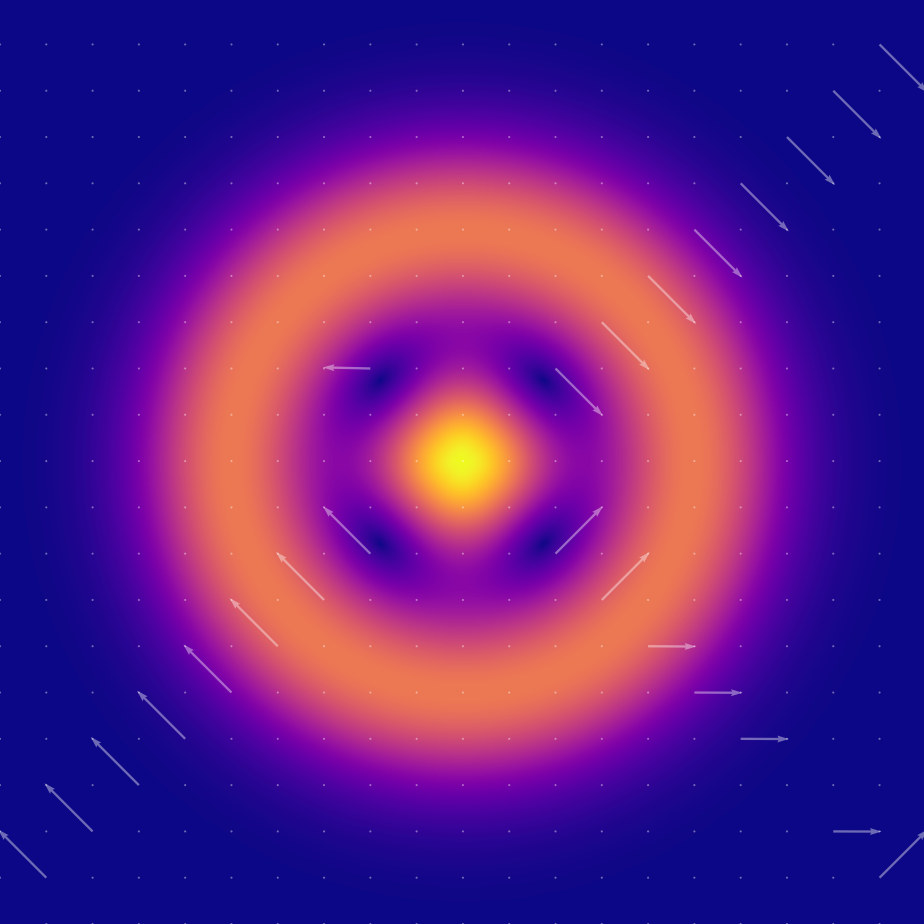
\includegraphics[width=0.48\textwidth]{figures/xi_higgs_ignition_overlay.png}
\caption{$\Xi$-Field Ignition: Higgs as the field ignition boundary. Compression of luxion wavefronts exceeds the mass-lock threshold, triggering a stable resonance node.}
\label{fig:higgs_field}
\end{figure}

\paragraph{GCFT Rupture Equation (W/Z Event):}
Let $\Xi(r,t)$ be the local coherence field.  
A rupture occurs when the field tension $|\nabla\arg\Xi|^2$ exceeds a critical threshold $\tau_c$:
\[
|\nabla\arg\Xi|^2 \geq \tau_c \implies \Xi(r, t) \to \Xi(r, t) + \delta\Xi_{\text{rupture}}
\]
where $\delta\Xi_{\text{rupture}}$ is a short-lived, high-torsion pulse:
\[
\delta\Xi_{\text{rupture}} \sim A \exp\left(-\frac{(r - r_0)^2}{2\sigma^2}\right) e^{i(\omega t + \phi_0)}
\]
with $A$, $\sigma$, and $\omega$ set by the local field configuration and energy input.

The *lifetime* $\tau_{W/Z}$ is the field’s relaxation time to restore sub-critical tension:
\[
\tau_{W/Z} \sim \frac{1}{\gamma_{\text{decoh}}}
\]
where $\gamma_{\text{decoh}}$ is the local decoherence rate.

\begin{figure}[ht]
\centering
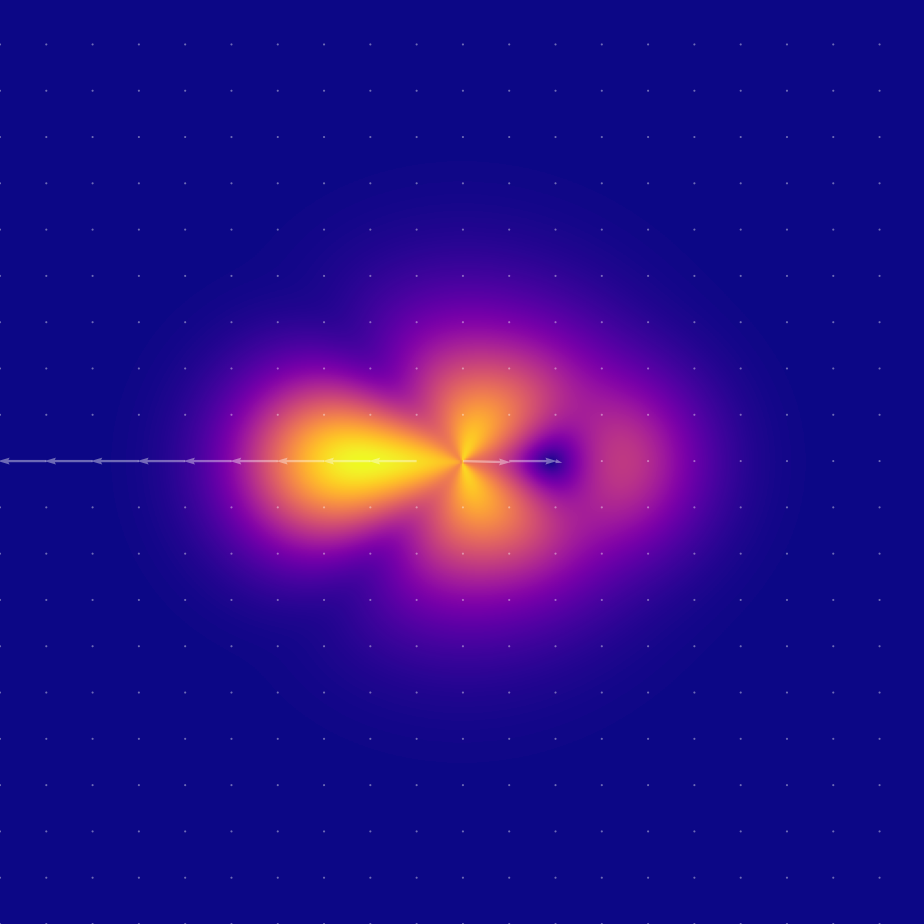
\includegraphics[width=0.48\textwidth]{figures/xi_wz_rupture_overlay.png}
\caption{$\Xi$-Field Torsion Lock: A simulated W/Z-like rupture in the $\Xi$ field. Localized chirality rebalancing results in short-lived coherence traps, visible as torsion swirls and phase cavities.}
\label{fig:wz_boson_field}
\end{figure}

\subsection{W and Z Bosons: Coherence Rupture States}

The W and Z bosons emerge at critical coherence tension levels where a $\Xi$-structure undergoes a topological phase transition. Rather than carrying a weak force, these structures are snapshots of field rupture—brief torsion traps during decoherence events like beta decay.

\begin{itemize}
  \item \textbf{W Boson}: Represents a chiral rupture—a directional tear in the coherence field causing local phase rebalancing. It mediates changes in charge only because the field structure reconfigures handedness.
  \item \textbf{Z Boson}: A symmetry-restoration lock—it forms when parity asymmetries resolve without charge transfer, trapping coherence before full unraveling.
\end{itemize}

These bosons appear and vanish not because they’re exchanged, but because the $\Xi$ field undergoes instability thresholds and quickly resettles.

\subsection{The Gluon: Phase Torsion Harmonizer}

In GCFT, the gluon is not a carrier of color charge. It is a phase torsion harmonizer: a local field twist that helps sustain coherent resonance between partial $\Xi$ nodes (traditionally interpreted as quarks). The strong force is not exchanged—it is the field's resistance to internal phase shearing.

\paragraph{GCFT Gluon Field Correction:}
Torsion in the coherence field:
\[
\vec{T}_\Xi = \nabla \times \nabla\arg\Xi
\]
In baryons, local field energy is minimized when torsion is harmonized:
\[
\mathcal{E}_{\text{baryon}} = \int \left( |\nabla\Xi|^2 + \alpha |\vec{T}_\Xi|^2 \right) dV
\]
with $\alpha$ a coupling parameter for torsion rigidity. No need for color charge or explicit gauge boson exchange; torsion “gluon” effects are collective field properties.

Gluon-like behavior emerges in dense compression knots (baryons), but only as a collective field correction. There is no need for eight color gluons. $\Xi$ symmetry does not fragment in this way.

\subsection{Boson Resonance Table}


\begin{table}[H]
\footnotesize
\centering
\begin{tabular}[t]{l c >{\raggedright\arraybackslash}p{3.5cm} c >{\raggedright\arraybackslash}p{3.5cm}}
\hline
\textbf{Boson} & \textbf{Mass (MeV)} & \textbf{GCFT Role} & \textbf{Stability} & \textbf{Observed as} \\
\hline
W$^\pm$    & 80,379   & Chiral rupture / handedness flip & Transient & Beta decay, lepton conversion \\
Z$^0$      & 91,188   & Parity lock / coherence trap     & Transient & Decay symmetry transition \\
Gluon ($g$)& 0        & Torsion harmonizer (not exchange, collective in baryons) & Collective, virtual & Baryon stability \\
Higgs ($H$)& 125,100  & Compression ignition (not a particle); boundary event; recoil artifact at threshold & Boundary event & Recoil artifact at threshold \\
Graviton   & --       & Not present (meaningless) & -- & -- \\
Photon ($\gamma$) & 0 & Luxion ripple (pure coherence pulse) & Stable (massless) & All EM field actions \\
\hline
\end{tabular}
\caption{GCFT boson reinterpretation: No boson is a force carrier; all are field rupture, ignition, or threshold states.}
\label{tab:boson_resonance_gcft}
\end{table}

\subsection{Gravity: Gradient of Field Compression}

The graviton is not only absent in GCFT—it is meaningless. Gravity arises as the macroscopic gradient of field compression:
\[
\vec{a}_{\text{gravity}} = -\nabla \Phi_\Xi
\]
where $\Phi_\Xi$ is the local coherence potential generated by luxion density:
\[
\Phi_\Xi(r) = \int \frac{\rho_\Xi(r')}{|r - r'|} d^3r'
\]
The curvature observed in spacetime is reinterpreted as a response to coherence imbalance. There is no need to quantize gravity, as there is no particle to quantize.

\subsection{Photon (Luxion): The Only Stable Bosonic Propagator}

In GCFT, the photon is a phase pulse—the sole bosonic excitation that propagates as a stable, massless ripple:
\[
\Xi_\gamma(r, t) = A \exp[i(k r - \omega t)]
\]
where $|\Xi_\gamma|^2$ is constant and $A$ is set by source compression. These are the fundamental coherence units (luxions), carrying phase but not mass.

\subsection{Summary and GCFT Predictions}

All GCFT bosons are \emph{threshold field states}. They reflect instabilities, rebalancing points, or local synchrony breakdowns in the $\Xi$ field. There is no exchange, no mediation—only resonance, tension, and collapse.

\paragraph{GCFT Predictions for Bosons:}
\begin{itemize}
  \item No isolated bosons can be observed except for photons (and possibly composite luxion modes in low-mass systems).
  \item The W/Z and Higgs appear only as short-lived field rupture events, not as true particles; their direct detection is always linked to rapid rebalancing of $\Xi$.
  \item Gluon "exchange" is a field correction in baryons only—no gluon jets outside hadrons, no color charge beyond local torsion harmonization.
  \item No graviton exists; gravity is phase gradient only. Any quantum of gravity detection would falsify GCFT.
  \item Collider events should show time delays, pre-chirps, or phase recoil signatures (coherence loss/rebound), not clean, long-lived bosonic propagation.
\end{itemize}

\subsection{Mapping to Standard Model Quantum Numbers}
\label{sec:sm_mapping}

Although GCFT replaces gauge symmetry with topological field coherence, many emergent behaviors traditionally attributed to SU(3) × SU(2) × U(1) symmetries still appear within the Ξ-field as geometric and phase constraints. The table below maps key Standard Model quantum numbers to their GCFT counterparts.

\begin{table}[H]
\centering
\resizebox{16cm}{!}{%
\begin{tabular}{lll}
\toprule
\textbf{SM Concept} & \textbf{GCFT Interpretation} & \textbf{Mechanism in $\Xi$} \\
\midrule
Color Charge (SU(3)) & Local phase node symmetry (triplet) & Torsion harmonization of 3-node $\Xi$-baryons \\
Weak Isospin (SU(2)) & Field reconfiguration parity & Knot-handedness and topological transitions \\
Hypercharge (U(1)) & Phase circulation bias & Net field winding number: $\oint \nabla \arg(\Xi)$ \\
Electric Charge & Chirality of torsion knot & Sign of local $\nabla \times \nabla \arg(\Xi)$ \\
Spin & Phase vortex circulation axis & Topological rotation of $\Xi$ field loops \\
Mass & Luxion compression & Local energy density of trapped phase curvature \\
\bottomrule
\end{tabular}%
}
\caption{Mapping of Standard Model gauge quantities to GCFT field-theoretic topologies.}
\label{tab:sm_gcft_mapping}
\end{table}

In this framework, the apparent success of gauge theories arises from the symmetry constraints enforced by stable Ξ-knot configurations. However, these are not fundamental symmetries of nature—they are emergent coherence lock conditions in a deformable, memory-bearing field. GCFT predicts that deviations from exact group behavior (e.g., anomalous decay paths, chirality flips under torsion stress) will become detectable in environments where phase coherence is disrupted or restructured.

